\documentclass{article}[12pt]
\title{\huge{\textbf{AIND Project 2\\Forward-Planning Agent}}}
\author{\Large{Ruize Luo}}

\usepackage{algorithm}
\usepackage[noend]{algpseudocode}
\usepackage[titletoc]{appendix}
\usepackage{amssymb}
\usepackage{amsmath}
\usepackage{amsthm}
\usepackage[english]{babel}
\usepackage{bm}
\usepackage{changepage}
\usepackage{geometry}
\usepackage{graphicx}
\usepackage{epstopdf}
\usepackage{enumerate}
\usepackage{enumitem}
\usepackage{extarrows}
\usepackage{hyperref}
\usepackage{indentfirst}
\usepackage{multirow}
\usepackage{tikz}
\usepackage{mathdots}
\usetikzlibrary{positioning,shapes,decorations.text, calc, backgrounds, decorations.pathmorphing}
\usepackage{float}
\usepackage{setspace}
\usepackage{subcaption}
\geometry{left=2.5cm,right=2.5cm,top=2.5cm,bottom=2.5cm}

\newcommand{\algind}{\hspace{\algorithmicindent}}
\newtheorem{theorem}{Theorem}
\newtheorem{lemma}{Lemma}
\newtheorem{definition}{Definition}

\tikzset{snake it/.style={-stealth,
		decoration={snake, 
			amplitude = .4mm,
			segment length = 2mm,
			post length=0.9mm},decorate}}

\newcommand{\ts}{Test\&Set }
\newcommand{\TS}{TEST\&SET }


\begin{document}
	\maketitle
	
	\section{Analysis of Results}
	
		\subsection{Number of Nodes Expanded vs Number of Actions in the Domain} \label{ssc:1.1}
			For the air cargo problem, there are three actions:
			\begin{itemize}
				\item $Load(Cargo, Plane, Airport)$
				\item $Unload(Cargo, Plane, Airport)$
				\item $Fly(Plane, Airport_1, Airport_2)$
			\end{itemize}
			
			Hence, given a problem with $C$ cargoes, $P$ planes and $A$ airports, we can calculate the number of possible actions:
			\begin{equation}
				N = 2(C \cdot P \cdot A) + P \cdot (A \cdot (A - 1))
			\end{equation}
			
			And hence we can calculate the number of actions for each of the four problems:
			\begin{center}
				\begin{tabular}{||c c c c c||} 
					\hline
					Problem & \# Cargoes & \# Planes & \# Airports & \# Actions \\ [0.5ex] 
					\hline\hline
					1 & 2 & 2 & 2 & \hphantom{0}20 \\ 
					\hline
					2 & 3 & 3 & 3 & \hphantom{0}72 \\
					\hline
					3 & 4 & 2 & 4 & \hphantom{0}88 \\
					\hline
					4 & 5 & 2 & 4 & 104 \\
					\hline
				\end{tabular}
			\end{center}
		
			Figure \ref{fig:n_actions_vs_n_nodes} is a plot of number of nodes expanded by each algorithm on each problem.
			
			\begin{figure}[h!]
				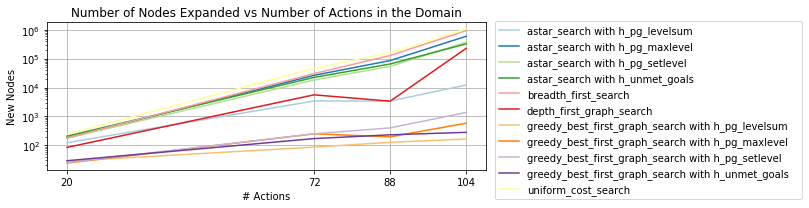
\includegraphics[width=\linewidth]{n_actions_vs_n_nodes.png}
				\caption{Number of nodes expanded vs number of actions in the domain for each search algorithm. Note that the y-axis is in log scale}
				\label{fig:n_actions_vs_n_nodes}
			\end{figure}
		
		
			From the graph we can see two things. Firstly, all algorithms show a log-linear relationship between number of nodes expanded and number of possible actions in the domain. The only differences among the algorithms are the slope of the line. Greedy algorithm seem to be looking into fewer new nodes than other algorithms.
			
			Secondly, there is a dip in number of nodes expanded for depth first graph search (DFS) and greedy best graph search with maxlevel heuristics when going from 72 actions to 88 actions. This might be due to the fact that problem 3 only has two planes whereas problem 2 had three, since now at most two planes can have actions at each expansion. This would reduce the branching factor and thus making it easier for DFS to find the solution.\\
			
		\subsection{Search Time vs Number of Actions in the Domain} \label{ssc:1.2}
		
			Below is a plot of search time for each algorithm on each problem.
			
			\begin{figure}[h!]
				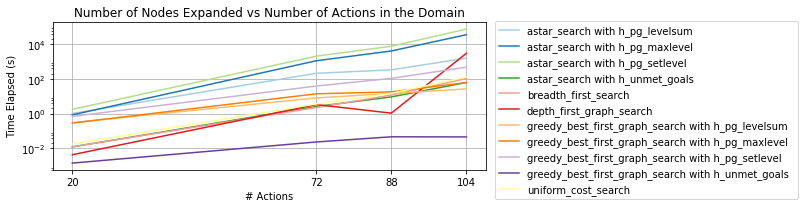
\includegraphics[width=\linewidth]{n_actions_vs_time.png}
				\caption{Search time (seconds) vs number of actions in the domain for each search algorithm. Note that the y-axis is in log scale}
				\label{fig:n_actions_vs_time}
			\end{figure}
			
			We can see that the relationship between search time is also approximately log-linear for all the algorithms. Greedy best first search with number of unmet goals heuristic outperforms other algorithms by being an order of magnitude faster. DFS has a steeper slope, which makes it suitable for very small problems (less than 20 actions).\\
			
		\subsection{Plan Length} \label{ssc:1.3}
			
			Below is a plot of plan length for each algorithm on each problem.\\
			
			\begin{figure}[h!]
				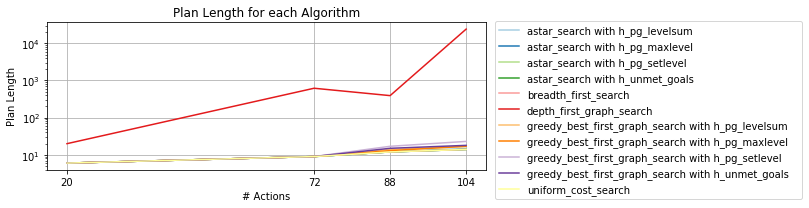
\includegraphics[width=\linewidth]{plan_length.png}
				\caption{Plan length for each search algorithm on each problem. Note that the y-axis is in log scale}
				\label{fig:plan_length}
			\end{figure}
		
			We can see that the path DFS plans is far from optimal and seems to be increasing faster than linear with number of actions even when the y-axis is already log-scale. In order to inspect the performance of the other algorithms, we should plot another one without DFS.
			
			\newpage
			\begin{figure}[h!]
				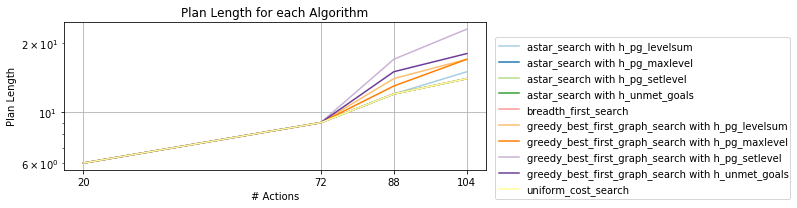
\includegraphics[width=\linewidth]{plan_length_no_dfs.png}
				\caption{Plan length for each search algorithm on each problem without DFS. Note that the y-axis is in log scale}
				\label{fig:plan_length_no_dfs}
			\end{figure}
		
			Note that there are 5 algorithms overlapping with the line that represents the shortest plan lengths for each problem:
			\begin{itemize}
				\item breadth first search (BFS)
				\item uniform cost search
				\item A* search with number of unmet goals
				\item A* search with maxlevel
				\item A* search with setlevel
			\end{itemize}
			
			We see that even though greedy best first search expands less nodes, A* searches with admissible heuristics find solutions that are optimal. Levelsum is not an admissible heuristic, and it did not find the optimal solution for problem 4.
			
	\section{Questions}
		
		\begin{enumerate}
			\item Which algorithm or algorithms would be most appropriate for planning in a very restricted domain (i.e., one that has only a few actions) and needs to operate in real time?
		\end{enumerate}
	
		\textit{Answer}: According to \ref{ssc:1.2}, DFS and greedy best first search with number of unmet goals heuristics operate the fastest under very restricted domains. However, DFS will become much worse if the domain ever expands.
		
		
		\begin{enumerate}[resume]
			\item Which algorithm or algorithms would be most appropriate for planning in very large domains (e.g., planning delivery routes for all UPS drivers in the U.S. on a given day)
		\end{enumerate}
	
		\textit{Answer}: Under very large domains, the storage requirement of the algorithms start to play a factor. Hence, ideally we would like algorithms where number of nodes expanded grows slowly with the size of the domain. As can be seen from the above analysis, greedy best first search algorithms brings about the best storage efficiency, while still having reasonable run time and being able to find reasonably good solutions.
		
	
		\begin{enumerate}[resume]
			\item Which algorithm or algorithms would be most appropriate for planning problems where it is important to find only optimal plans?
		\end{enumerate}
	
		\textit{Answer}: If optimality must be achieved, then A* with admissible heuristic, BFS and uniform cost search can be used (as listed in \ref{ssc:1.3}). 
	
	
\end{document}\textbf{}